
\newpage
\section{Fase 4}
\label{sec:Fase4}

We voegen tijdens fase 4 nog een laatste spel toe. Arkanoid (figuur: \ref{fig:akranoid}) is een spel waar je enkel met de joystick speelt. De enige bewegingen die daarbij gemaakt worden is naar links en rechts. Doordat het kan zijn dat de bal boven de blokken eventjes blijft. De joystickmovements zullen dus een pak minder zijn dan andere spelletjes. Doordat er ook geen knoppen gebruikt worden zal het algoritme deze 2 spelletjes het moeilijkst uit elkaar kunnen worden want Pacman heeft gelijkaardige waarden. 

\begin{figure}[]
	\centering
	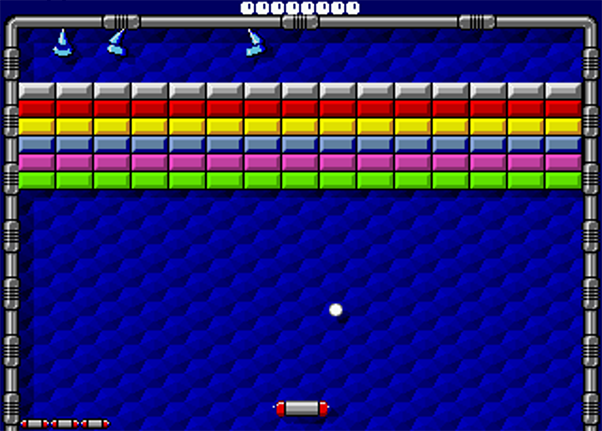
\includegraphics[width=0.6\textwidth]{img/arkanoid.png}
	\caption{Het 4de spel in de dataset}
	\label{fig:akranoid}
\end{figure}

\subsection{Logistische regressie}
\label{sec:Logistischeregressie-fase4}

Qua implementatie hoeft er niets te veranderen dus die blijft dezelfde als in code \ref{code:logistischeregressiefase3}. We gaan nu ook direct door naar de vijf inputparameters omdat die het meest aanleunen bij de realiteit. 

\subsubsection{Resultaten}
\paragraph{Snelheid van het algoritme} 

\paragraph{Foutratio} 

Nu we met meerdere klassen werken is het niet meer mogelijk om de F-score te berekenen omdat die enkel kan berekend worden tussen binaire classificaties. Onze testdataset telt nu 150 voorbeelden doordat er 50 extra voorbeelden van Tetris zijn toegevoegd. We laten het leeralgoritme stoppen wanneer een tolerance van 0.1 bereikt is. Bij eerste test met twee inputparameters beslist logistische regressie 143 van de 150 voorbeelden correct. Van de foutieve voorspellingen dacht het algoritme vijf maal dat Tetris gespeeld werd en een twee keer Pacman terwijl het eigenlijk zeven keer Mortal Kombat moest zijn. 

Wanneer er drie inputvectors gebruikt worden dan voorspelt het algoritme even veel voorbeelden fout maar nu denkt hij vier keer dat Mortal Kombat gespeeld werd ipv Pacman. De andere drie fouten gebeuren bij het verschill tussen Tetris en Mortal Kombat waar hij telkens de voorkeur geeft aan Tetris.

De volgende test met vijf inputvectors maakt acht foutieve voorspellingen. Waarvan vier keer de voorspelling Mortal Kombat Pacman had moeten zijn. Twee keer kreeg Tetris de voorkeur op Mortal Kombat net als dat Pacman twee keer daar de voorkeur op kreeg.


\newpage
\subsection{Support Vector Machine}
\label{sec:supportvectormachineFase4}
Ook voor de Support Vector Machine is de implementatie gewijzigd. U kan de code zien in figuur We maken gebruik van de lineaire kernel wat eigenlijk de standaard kernel is voor SVMs.


\subsubsection{Resultaten}
\paragraph{Snelheid van het algoritme} 
Een probleem die zich voordoet bij de Support Vector Machines is dat het aantal iteraties niet kunnen vastgezet worden. De Tolerance kunnen we wel wijzigen maar gelijk welke waarde we daar aan toekennen, de snelheid blijft hetzelfde. Dit zal waarschijnlijk een fout zijn in het Accord-framework. Of er nu 2, 3 of 5 inputvectoren zijn, de gemiddelde tijd van het leerproces is 135,0201 ms.


\paragraph{Foutratio}
Ook de Support Vector Machine blijft niet foutloos in deze fase tot en met 3 inputparameters is het algoritme wel nog feilloos vanaf vier worden er 2 spelletjes foutief voorspelt.  

\subsection{Conclusie na fase 3}
Ondanks dat we de snelheid niet precies met elkaar kunnen vergelijken zien we toch wel dat een Support Vector Machine meer tijd nodig heeft dan logistische regressie. We kunnen dit ook staven. We weten dat de tijd van een SVM met vijf inputvectors er gemiddeld 135,0201 ms over doet maar dan zijn er wel 2 foute voorspellingen. Om een perfect algoritme te krijgen zal het dus nog beetje langer dan 135,0201 ms duren. De tijd van een logistische regressie met vijf inputparameters bedraagt 66,7429 ms en dan is het algoritme foutloos. Dus op die manier weten we zeker dat het algoritme van SVM langer duurt dan logistische regressie. 

Bij het foutratio zien we dan wel dat de SVM beter presteert dan logistische regressie met slecht 2 fouten tegenover 7. 

 